\section {Carboxylic Acid Solvation}

To address solvation of the carboxylic head groups, we have calculated the O-O and O-H atomic pair correlations to generate the radial distribution functions (RDF) of Figure \ref{fig:rdfs}. RDF plots of the two carboxylic acid oxygens are shown designated as ``alc'' and ``carb'' referring to the alcohol and carbonyl moieties of the acid head groups. The RDFs show the correlations with distance to neighboring water oxygens and hydrogens, labeled accordingly.

Each plot of Figure \ref{fig:rdfs} is a depth profile represented as a series of RDFs that correspond to different depths from the surface. The plots vary from dark blue to bright red, corresponding to a transition from -12\angs~to +2\angs~positions relative to the surface location, respectively, with negative values located further into the water bulk. The location of the molecule was calculated based on the molecular center of mass. This depth-profiling allows for evaluation of the water structure around the carboxylic acid head groups as a function of depth under the water surface.

\begin{figure}[h!]
	\begin{center}
		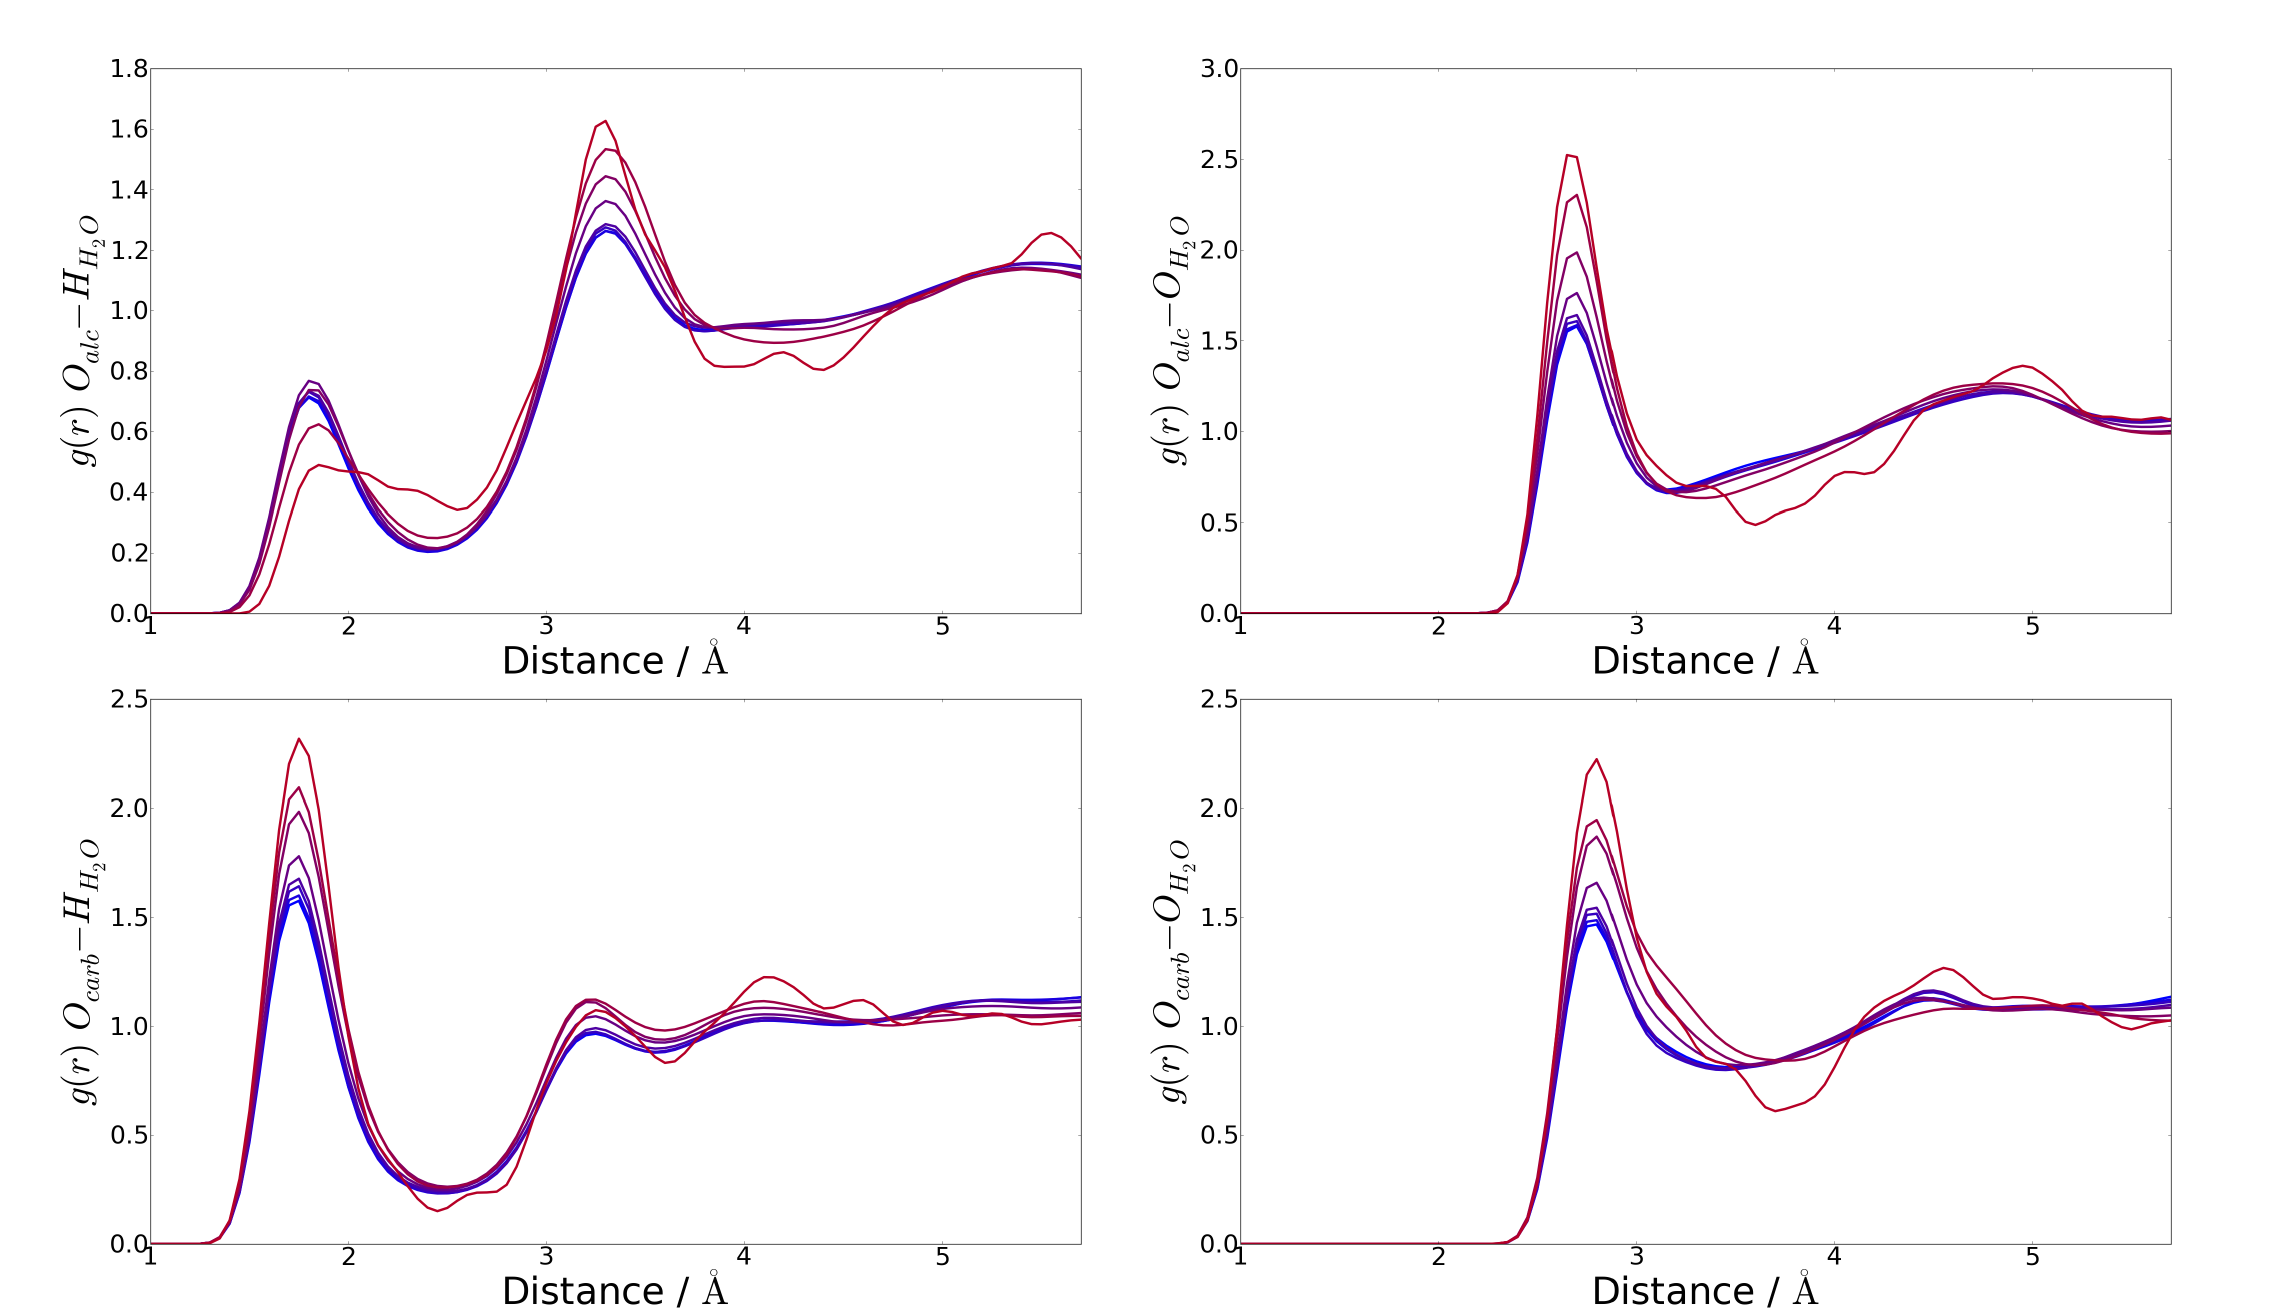
\includegraphics[scale=1.0]{images/rdf/rdf-collection.png}
		\caption{}
		\label{fig:rdfs}
	\end{center}
\end{figure}

The right column of plots in Figure \ref{fig:rdfs} shows the RDFs of the O$_{carbonyl}$ and O$_{alcohol}$ correlated to water oxygens. Peak locations are similar for both RDFs. The trend with increasing depth is a decrease in structure of the water oxygens around the acid oxygens. Overall, there is similarity between the two plots, except for a slightly larger first peak around the alcohol oxygen. The alcohol group bonds with both water oxygen and hydrogens, whereas the carbonyl only attracts hydrogens. The increase of the RDF intensity as the succinic acid moves further towards the surface out of the water bulk is notable. This indicates a stronger structuring of waters and tighter binding between the acid group and surface waters as the molecule moves closer to the gas-side of the interface.

The two plots in the left column of Figure \ref{fig:rdfs} show the RDFS of acid oxygens correlated to water hydrogens. Clearly the carbonyl oxygen binds more of the water hydrogens with a first peak that is nearly three times taller than the alcohol oxygen. While the carbonyl RDF increases with positions closer to the gas phase side of the surface, the alcohol-oxygen - water-hydrogen RDF decreases in the uppermost positions just at, or slightly above the surface in the gas phase. The alcohol oxygen has weaker binding to water hydrogens and it further weakens as the acid reaches the topmost layer of the surface. This is most likely due to the acid orientation at the surface, and will be examined later in this work.


